\section{Introduction}

The Cell Broadband Engine $^{TM}$ (Cell BE) processor \cite{DP05} is now
commercially available in both the Sony PS3 game console and the IBM BladeCenter
which represents the first product on its development road-map. The
anticipated high volumes for this non-traditional commodity hardware continue
to make it interesting in a variety of different application spaces, ranging
from the obvious multi-media and gaming domain, through the HPC space (both
traditional and commercial), and to the potential use of Cell as a building
block for very high end supercomputing systems \cite{Wil06}. 

This first generation Cell processor provides flexibility and performance
through the inclusion of a 64-bit multi-threaded Power Processor $^{TM}$
Element (PPE) with two levels of globally-coherent cache and support for
multiple operating systems including Linux. For additional performance, a Cell
processor includes eight Synergistic Processor Elements (SPEs), each consisting
of a Synergistic Processing Unit (SPU), a 256K local memory,
and a globally-coherent DMA engine.
Computations on the SPUs are performed by 128-bit wide Single Instruction
Multiple Data (SIMD) functional units. An integrated high bandwidth bus, the
Element Interconnect Bus (EIB), glues together the nine processors and their
ports to external memory and IO, and allows the SPUs to be used for streaming
applications \cite{MG06}.

Data is transferred between the local memory and the DMA engine \cite{Kis06} in
chunks of 128 bytes. The DMA engine can support up to 16 concurrent requests of
up to 16K bytes originating either locally or remotely. The DMA engine is part
of the globally coherent memory address space; addresses of local DMA requests
are translated by a Memory Management Unit (MMU) before being sent on the bus.
Bandwidth between the DMA and the EIB bus is 8 bytes per cycle in each
direction. Programs interface with the DMA unit via a channel interface and
may initiate blocking as well as non-blocking requests.

Programming the SPE processor is significantly enhanced by the
availability of an optimizing compiler which supports SIMD intrinsic
functions and automatic simdization \cite{AE03}. However, programming
the entire Cell processor consisting of the coupled PPE and 8 SPE
processors is a much more complex task, requiring partitioning of an
application to accommodate the limited local memory constraints of the
SPE, parallelization across the multiple SPEs, orchestration of data
transfers through insertion of DMA commands, and compiling for two
distinct ISAs.

To help users to harness such a powerful yet complicated processor and to port
existing legacy code, we developed an OpenMP\cite{Ope05} implementation for the
system. This is the same as a typical OpenMP implementation such as in Figure
\ref{fig:runtime}.

In this figure, the language-dependent frontends will translate user
source code to an \emph{intermediate representation (IR)}, to be
processed by an optimizing compiler into a resulting \emph{node
program}, which interacts with a \emph{runtime} environment that
starts and controls the multi-threaded execution.

\begin{figure}[!h]
  \begin{center}
    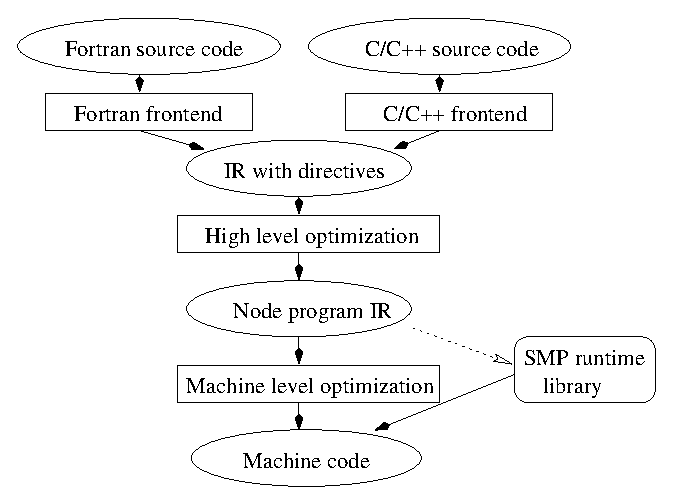
\includegraphics[angle=0, width=0.70\textwidth]{runtime.eps}
    \caption{\footnotesize Compiler and runtime structure}
    \label{fig:runtime}
  \end{center}
\end{figure}

With this system, the programming the Cell processor can benefit from
an industry standard in a familiar user environment. The compiler
will:

\begin{itemize} 

\item \textbf{Systematically manage multiple SPU threads} Users do not need to
  know Cell SDK details, as thread management on the SPUs is
  provided through the OpenMP framework.

\item \textbf{Automatically overlap computation and communication} The compiler
will generate data communication between the PPU main memory and the SPU
local store. DMA buffering and software cache can be automatically used to exploit
the large bandwidth between main memory and all 9 processors.

\item \textbf{Enlarge the limited SPU address space} Our OpenMP Cell
  compiler will treat SPU local storage more like a cache in a traditional
  processor. Large application data and code will be kept in the
  main memory of the PPU and paged in or transfered as appropriate.

\end{itemize}

%This is a common strategy used by many previous works $need more$
%\cite{lcpc97}.

There are already papers introducing the second and the third points\cite{Br07}
of the system, but little discussion has been dedicated to the OpenMP runtime
environment itself. The OpenMP standard continues to evolve and there
are still many open issues in this area, including the mechanisms required to
support nested parallelism, task, and more.

In this paper, we will focus on the first item, the major runtime environment
implementation itself\footnote{Topics such as threadprivate and C++ object
privatization will be discussed elsewhere.}.

The runtime system we have developed is based on the OpenMP
runtime library we use for other XL series compilers, including C/C++
and Fortran on AIX\copyright and Linux systems \cite{Zha04}. This paper
shows how to map the OpenMP environment to the Cell system. It
concentrates on discussions of the implementation considerations,
rather than implementation details. Some performance numbers are also
given.

%General speaking, the amount of thread local storage can not be
%determined statically. Because it is not clear at compile time that how
%many threads will be created to execute the OpenMP program. The total
%amount of memory used is better to be decided at run time dynamically.
